\chapter{APPENDICES}

\section{Project Schedule}
\begin{figure}[H]
	\centering
	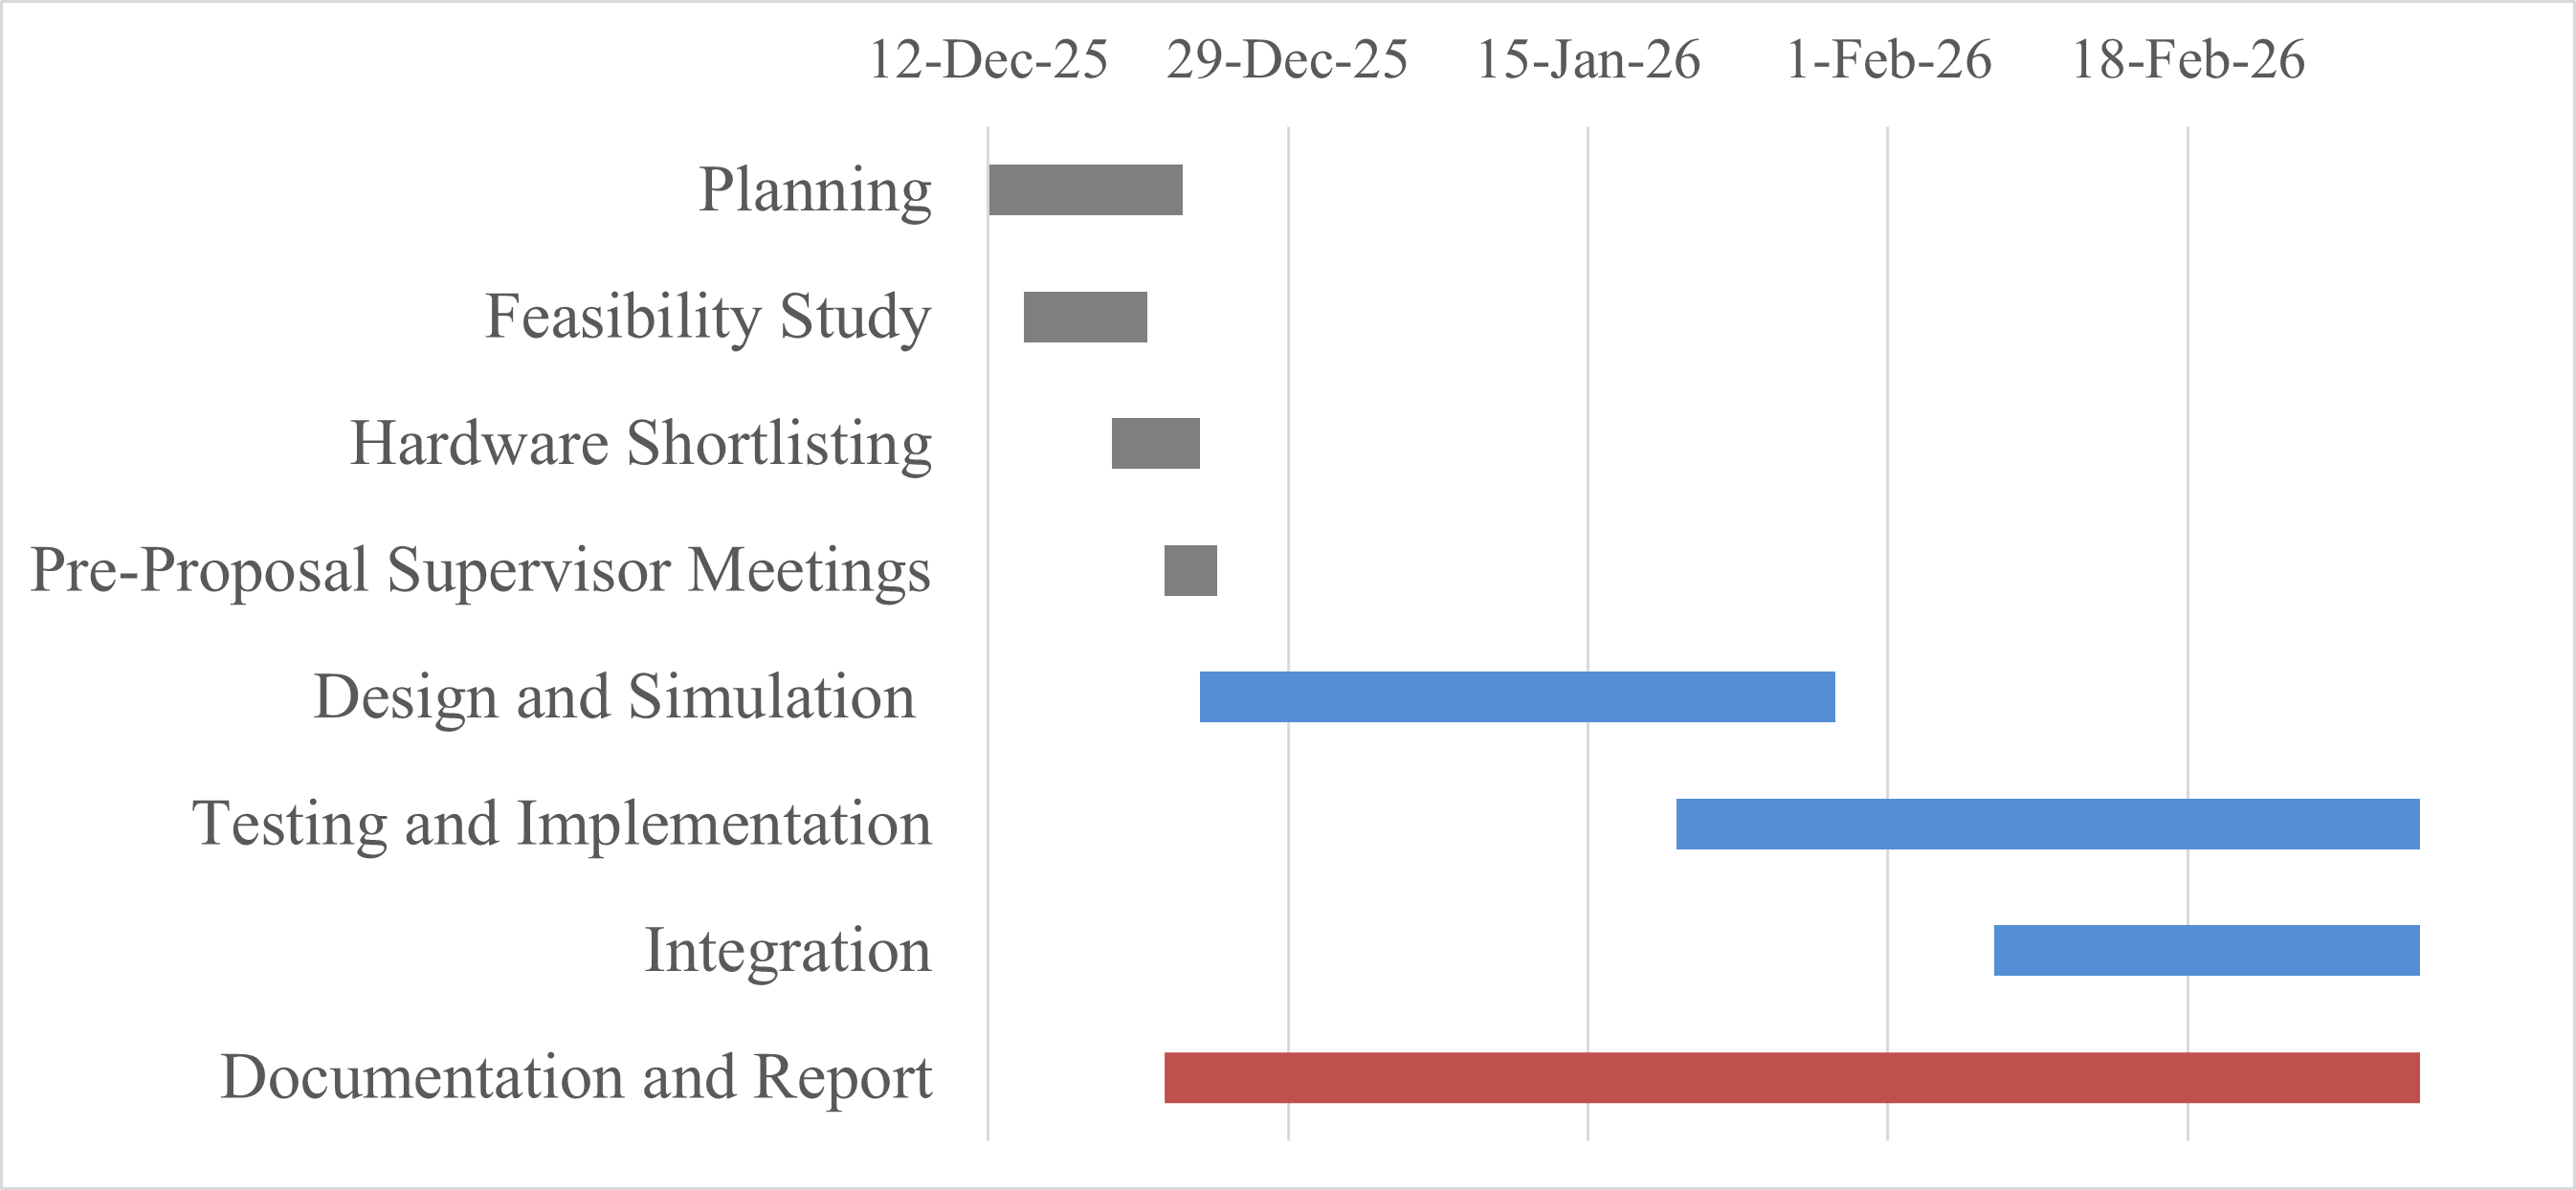
\includegraphics[width=\textwidth]{src/images/figures/gantt_chart.png}
	\caption{Project Gantt Chart}
	\label{gantt_chart}
\end{figure}
\newpage

\section{Budget Estimation}
\begin{table}[H]
	\centering
	\caption{Bill of Materials for EEG Acquisition Module}
	\begin{tabular}{|p{7.5cm}|c|c|c|}
		\hline
		\textbf{Component} & \textbf{Qty} & \textbf{Unit Cost} & \textbf{Total Cost} \\
		\hline
		Arduino Uno & 1 & 1000 & 1000 \\
		\hline
		AD620 Instrumentation Amplifier Module & 1 & 700 & 700 \\
		\hline
		LM741 Op-Amp IC & 3 & 40 & 120 \\
		\hline
		10~nF Capacitors & 5 & 10 & 50 \\
		\hline
		22~nF Capacitors & 5 & 10 & 50 \\
		\hline
		47~nF Capacitors & 5 & 10 & 50 \\
		\hline
		100~nF Capacitors & 5 & 10 & 50 \\
		\hline
		Resistor Box (Bundle of Resistors) & 1 & 175 & 175 \\
		\hline
		Gold Cup EEG Electrodes & 3 & 700 & 2100 \\
		\hline
		12~V Power Supply & 1 & 200 & 200 \\
		\hline
		Miscellaneous\textsuperscript{*} &  &  & 1000 \\
		\hline
		\multicolumn{3}{|r|}{\textbf{Total}} & \textbf{5495} \\
		\hline
	\end{tabular}
	\label{bill_of_materials}
\end{table}

\newpage
\section{Circuit Diagram}
\begin{figure}[H]
	\centering
	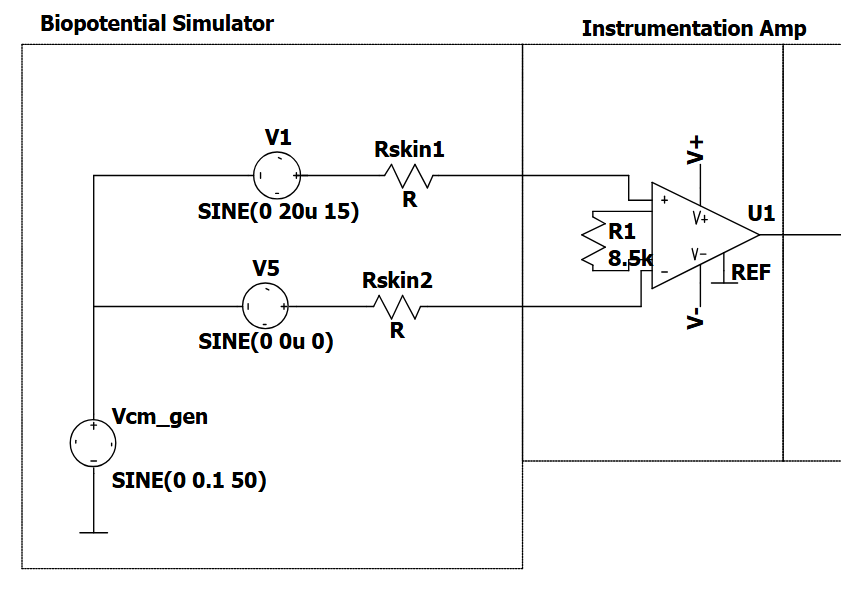
\includegraphics[width=\textwidth]{src/images/figures/ad620.png}
	\caption{AD620 (Instrumentation Amplifier)}
	\label{ina}
\end{figure}

\begin{figure}[H]
	\centering
	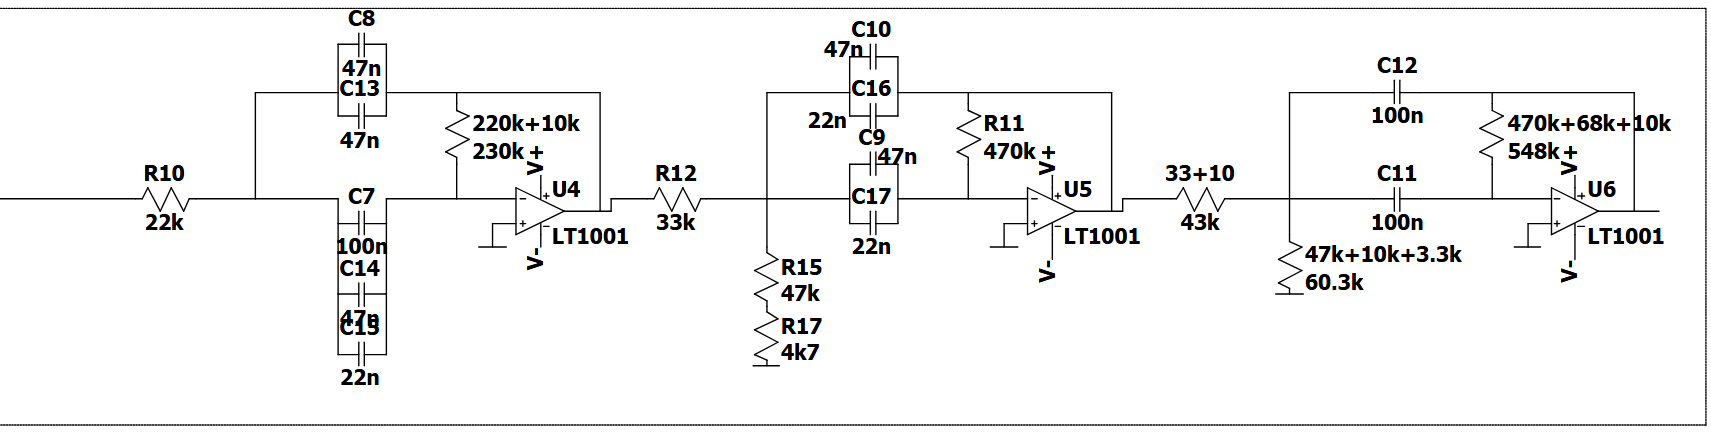
\includegraphics[width=20cm, height=7.5cm, angle = 90]{src/images/figures/filter_stage.png}
	\caption{$6^{\text{th}}$ order butterworth filter using lm741}
	\label{filter_circuit}
\end{figure}

\begin{figure}[H]
	\centering
	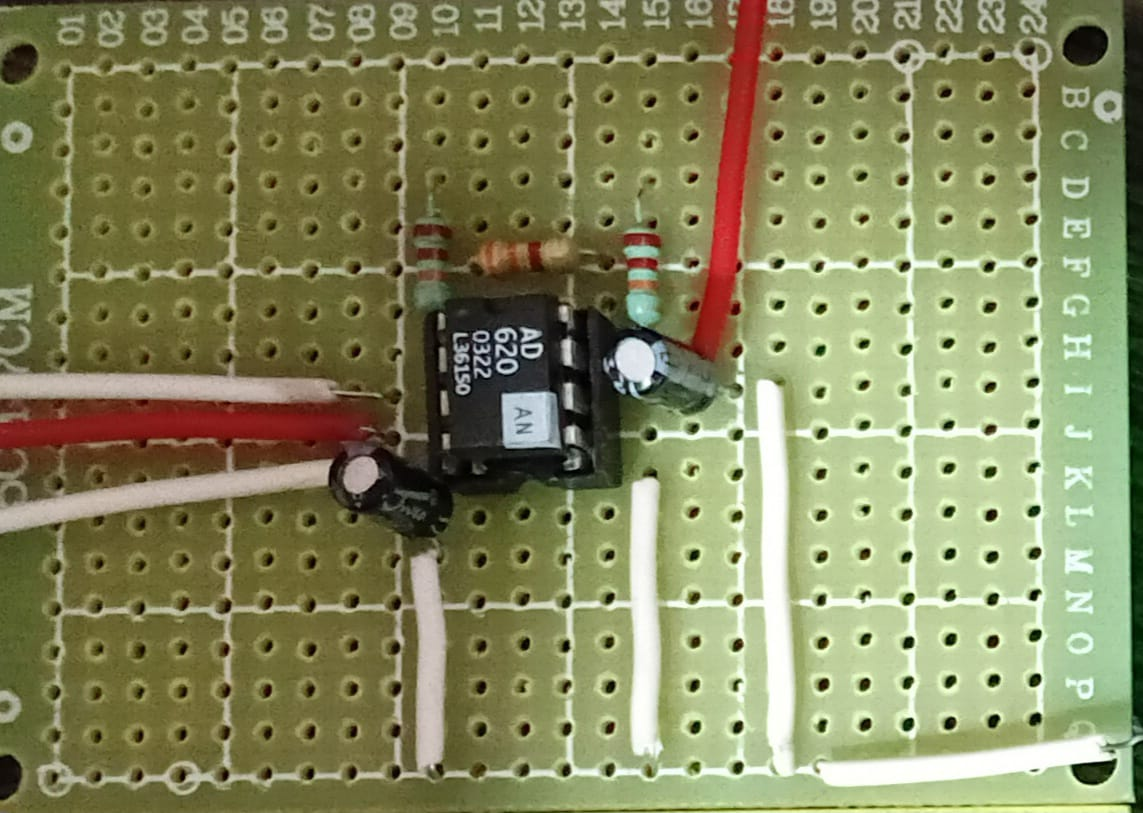
\includegraphics[width=10cm, height=7.5cm]{src/images/figures/ad620_h.jpg}
	\caption{AD620 Instrumentation Amplifier Circuit}
	\label{ad620_h}
\end{figure}

\begin{figure}[H]
	\centering
	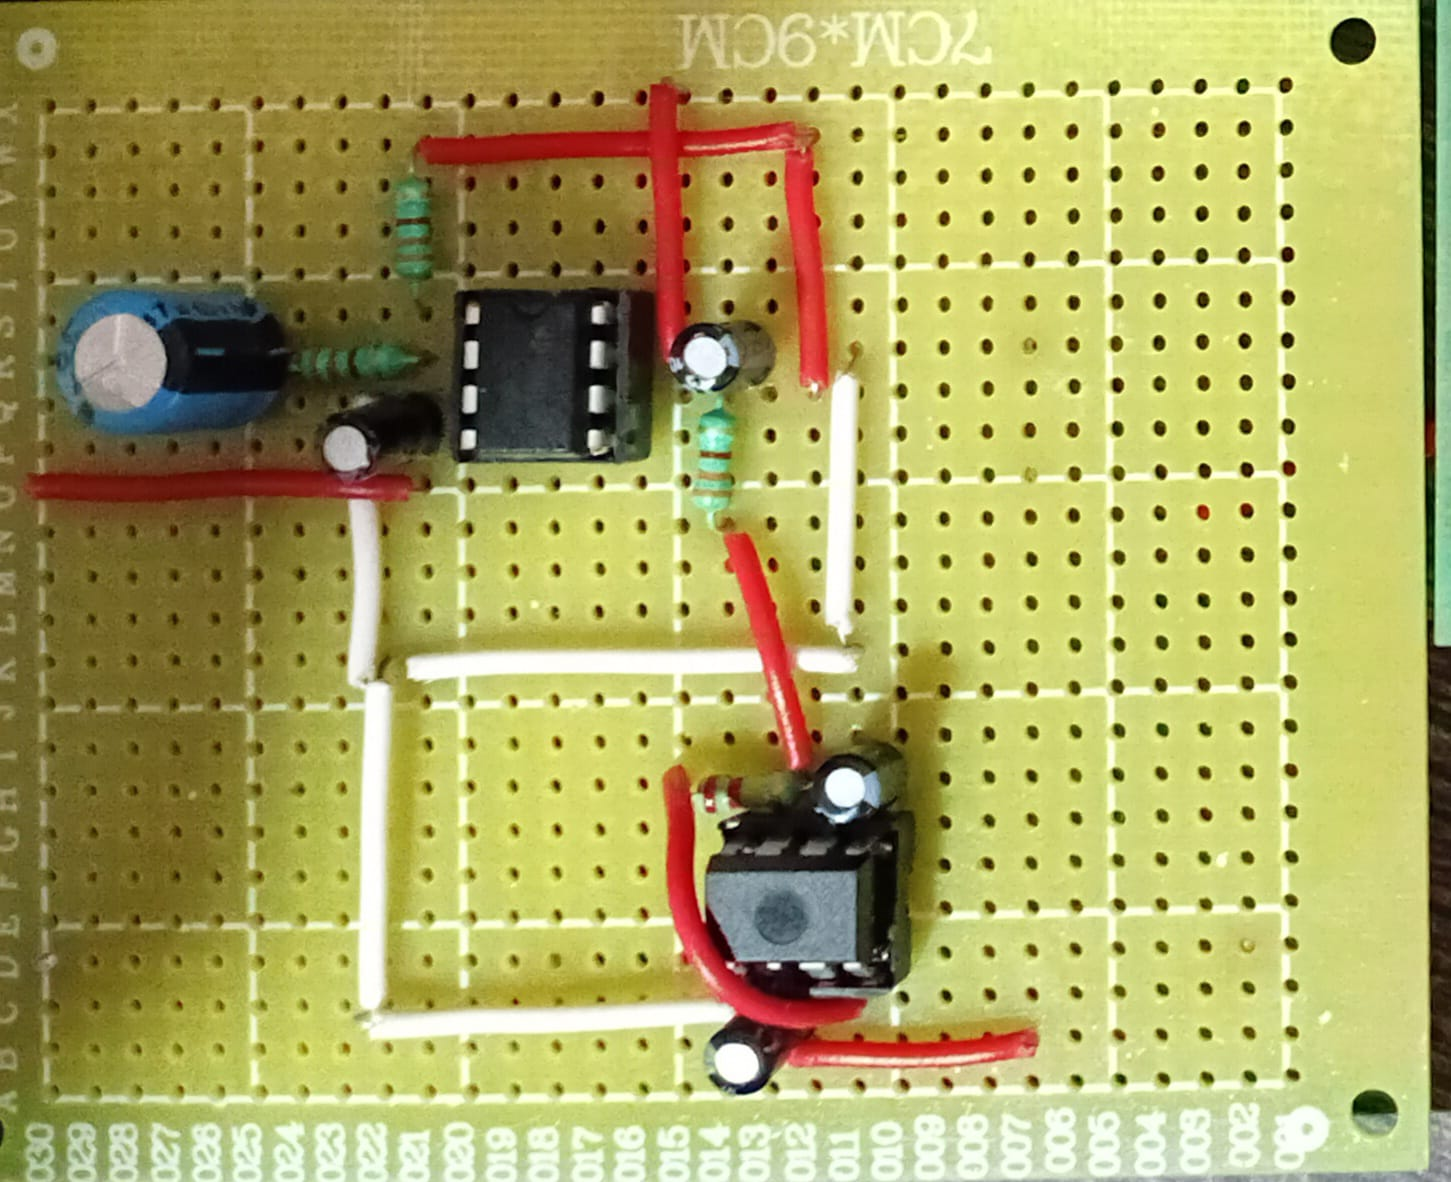
\includegraphics[width=10cm, height=7.5cm]{src/images/figures/high_pass_h.jpg}
	\caption{High Pass Filter Circuit}
	\label{high_pass_h}
\end{figure}

\begin{figure}[H]
	\centering
	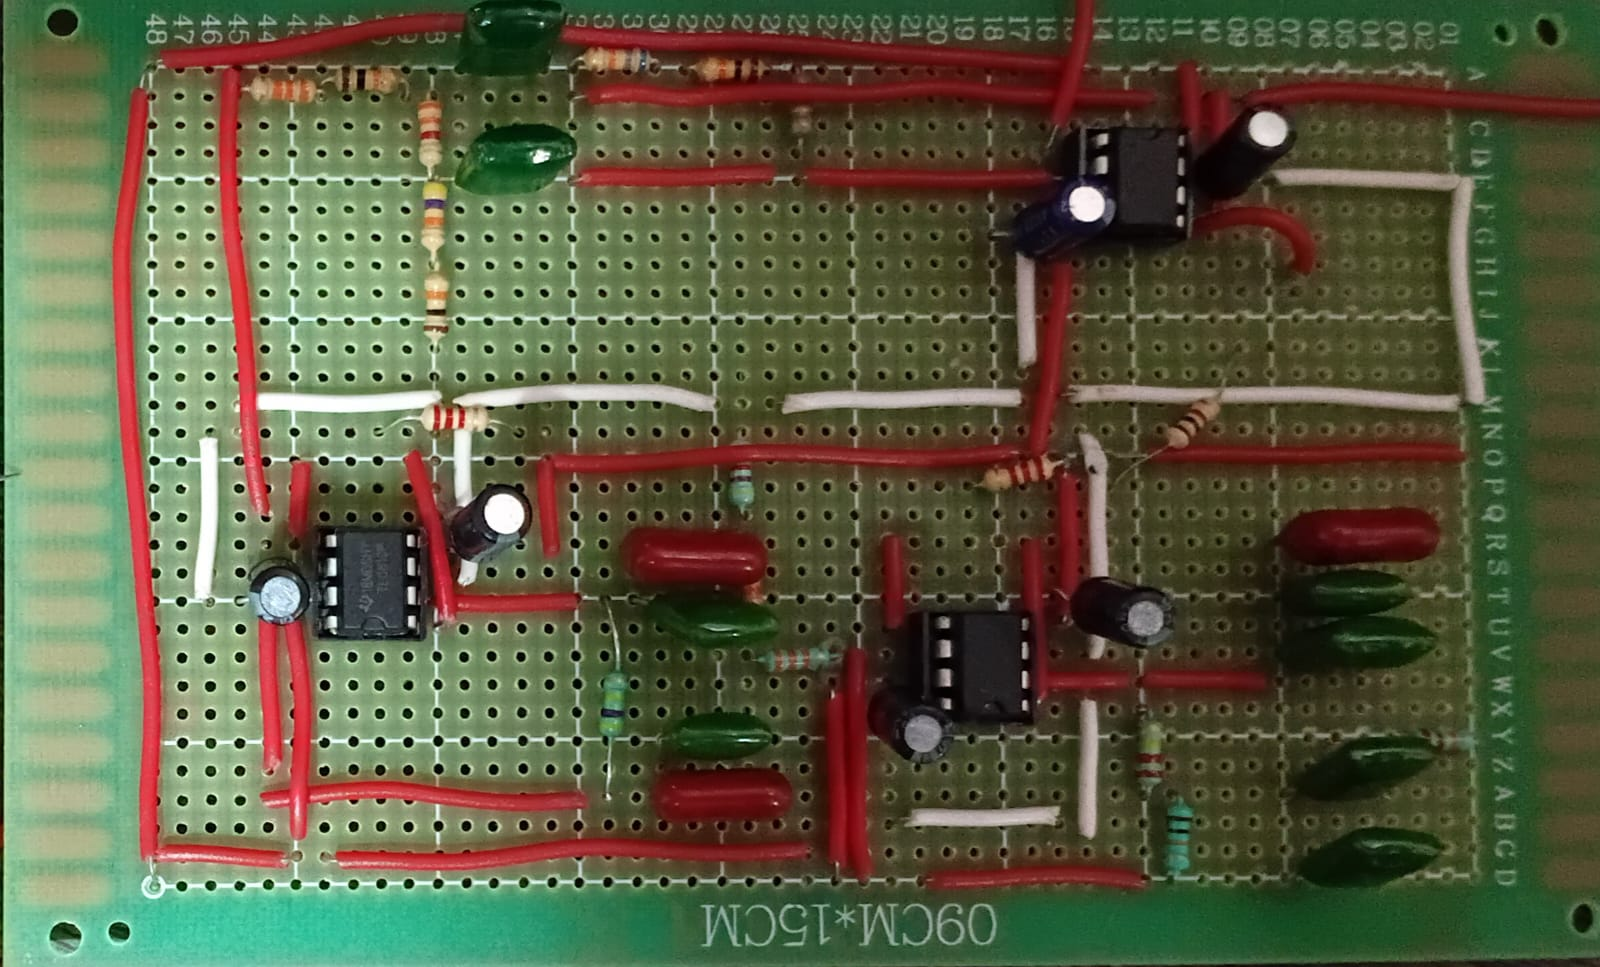
\includegraphics[width=10cm, height=7.5cm]{src/images/figures/3stage_h.jpg}
	\caption{Three Stage $6^{\text{th}}$ Order Band Pass Circuit}
	\label{3stage_h}
\end{figure}

\begin{figure}[H]
	\centering
	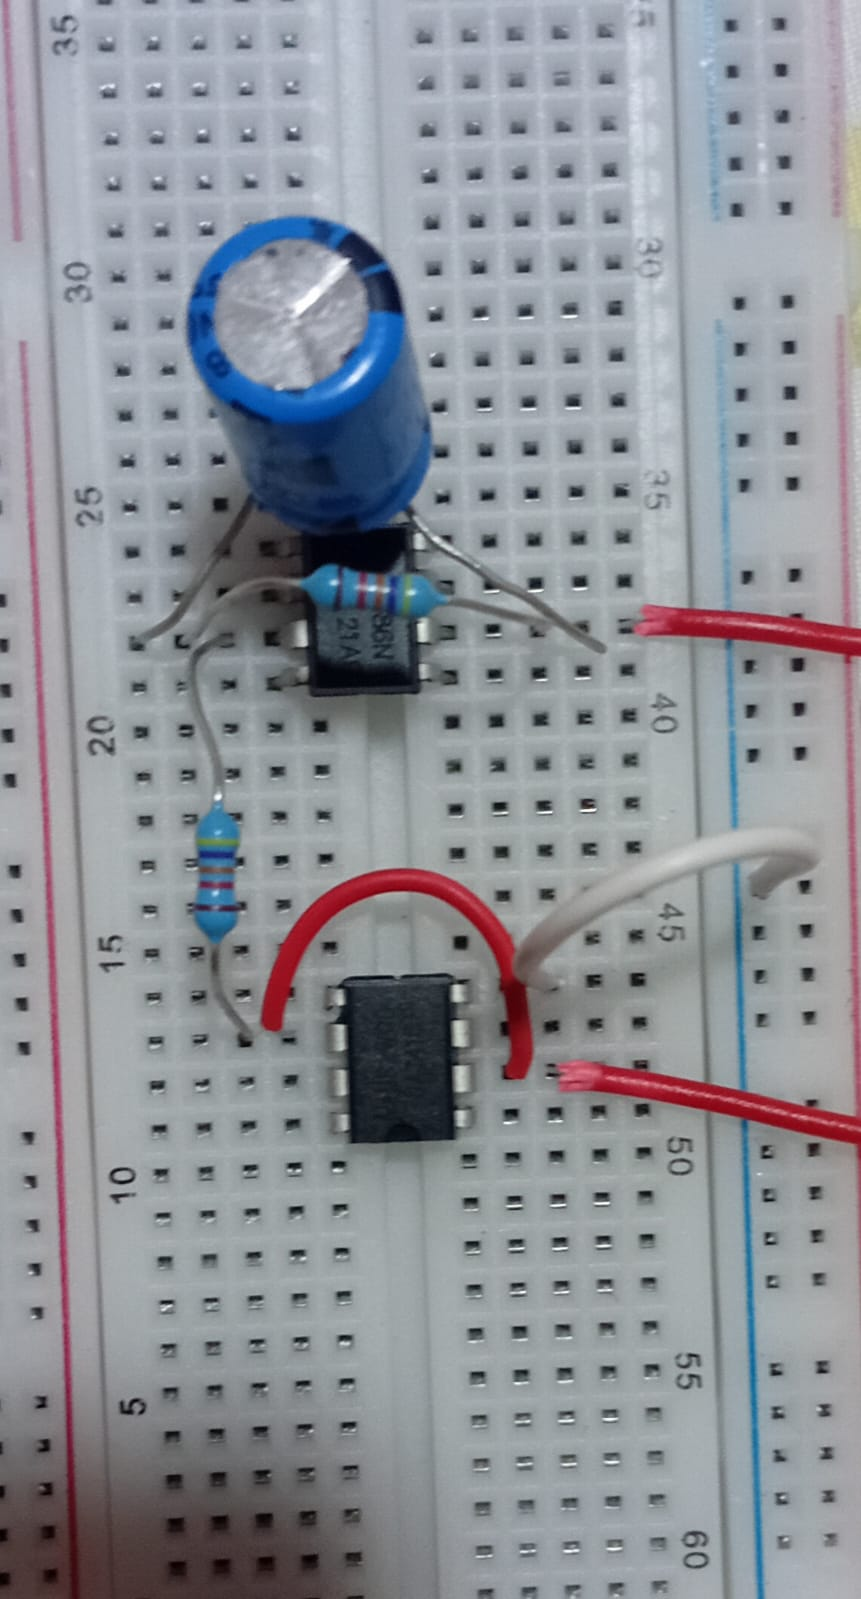
\includegraphics[width=10cm, height=7.5cm]{src/images/figures/drl_h.jpg}
	\caption{DRL Circuit}
	\label{drl_h}
\end{figure}


\newpage
\section{Module Specifications}

\subsection{EEG Signal Acquisition Module}
\begin{table}[H]
	\centering
	\small
	\caption{EEG Signal Acquisition Module}
	\begin{tabular}{p{6.5cm}p{6.5cm}ccc}
		\toprule
		\textbf{Parameter}                  & \textbf{Specification}   							\\
		\midrule
		Signal Type                     	& Electroencephalogram (EEG)						\\
		Number of Electrodes                & 3 (Fp1, Fp2, Reference)     						\\
		Electrode Type						& Ag/AgCl Surface Electrodes 						\\
		Input Signal Amplitude				& \SI{10}{\micro\volt} - \SI{100}{\micro\volt} 		\\
		Frequency 							& 0.5Hz - 40Hz 										\\
		Mode of Acquisition 				& Non invasive				 						\\
		\bottomrule
	\end{tabular}
	\label{eeg_signal_acq_module}
\end{table}


\subsection{Instrumentation Amplifier Module (AD620)}
\begin{table}[H]
	\centering
	\small
	\caption{Instrumentation Amplifier Module (AD620)}
	\begin{tabular}{p{6.5cm}p{6.5cm}}
		\toprule
		\textbf{Parameter} & \textbf{Specification} \\
		\midrule
		IC Used & AD620 \\
		Input Impedance & $\geq$ \SI{10}{\giga\ohm} \\
		CMRR & > 100 dB \\
		Gain Equation & \( G = 1 + \frac{49.4~\text{k}\Omega}{R_g} \) \\
		Supply Voltage & ±9 V \\
		Application & Low-level biopotential amplification \\
		\bottomrule
	\end{tabular}
\end{table}

\subsection{Signal Conditioning Module (Filters)}
\begin{table}[H]
	\centering
	\small
	\caption{Signal Conditioning Module (Filters)}
	\begin{tabular}{p{6.5cm}p{6.5cm}}
		\toprule
		\textbf{Filter Type} & \textbf{Specification} \\
		\midrule
		High-Pass Filter & Cut-off frequency = \SI{10}{\hertz} \\
		Low-Pass Filter & Cut-off frequency = \SI{40}{\hertz} \\
		Filter Order & Second order \\
		Purpose & Noise and artifact removal \\
		\bottomrule
	\end{tabular}
\end{table}

\subsection{Data Acquisition and Processing Module Specifications}
\begin{table}[H]
	\centering
	\small
	\caption{Data Acquisition and Processing Module Specifications}
	\begin{tabular}{p{6.5cm}p{6.5cm}}
		\toprule
		\textbf{Parameter} & \textbf{Specification} \\
		\midrule
		Microcontroller & Arduino Uno \\
		ADC Resolution & 10-bit \\
		Sampling Frequency & \SI{256}{\hertz} - \SI{1024}{\hertz} \\
		Input Voltage Range & 0 – 5 V \\
		Communication & USB Serial \\
		\bottomrule
	\end{tabular}
\end{table}

\subsection{EEG Signal Processing Module Specifications}
\begin{table}[H]
	\centering
	\caption{EEG Signal Processing Module Specifications}
	\begin{tabular}{p{5.5cm}p{8cm}}
		\toprule
		\textbf{Parameter} & \textbf{Specification} \\
		\midrule
		Programming Language & MATLAB \\
		Signal Processing & FFT based frequency analysis \\
		EEG Bands Analyzed & Beta Waves (10-30 Hz) \\
		Blink Detection & Amplitude threshold based \\
		Output & Text selection control \\
		\bottomrule
	\end{tabular}
	\label{tab:eeg_signal_processing}
\end{table}

\newpage

\section{Keyboard Interface}
\begin{figure}[H]
	\centering
	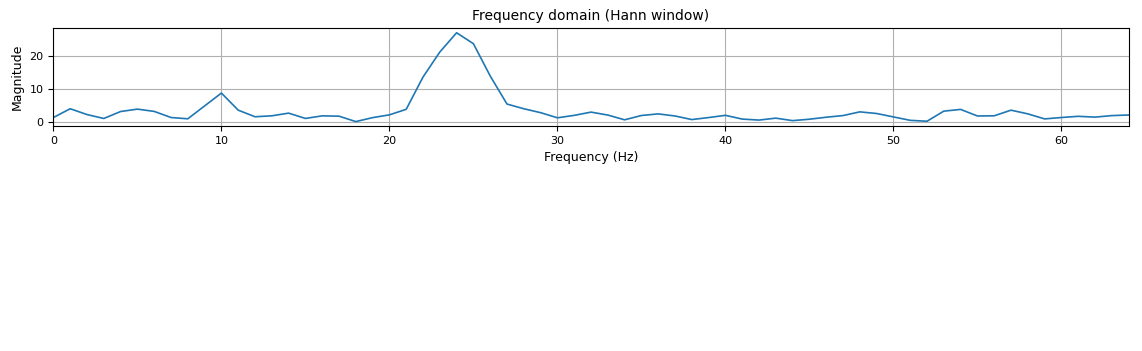
\includegraphics[width=\textwidth]{src/images/figures/keyboard_1.png}
	\label{keyboard_1}
\end{figure}
\begin{figure}[H]
	\centering
	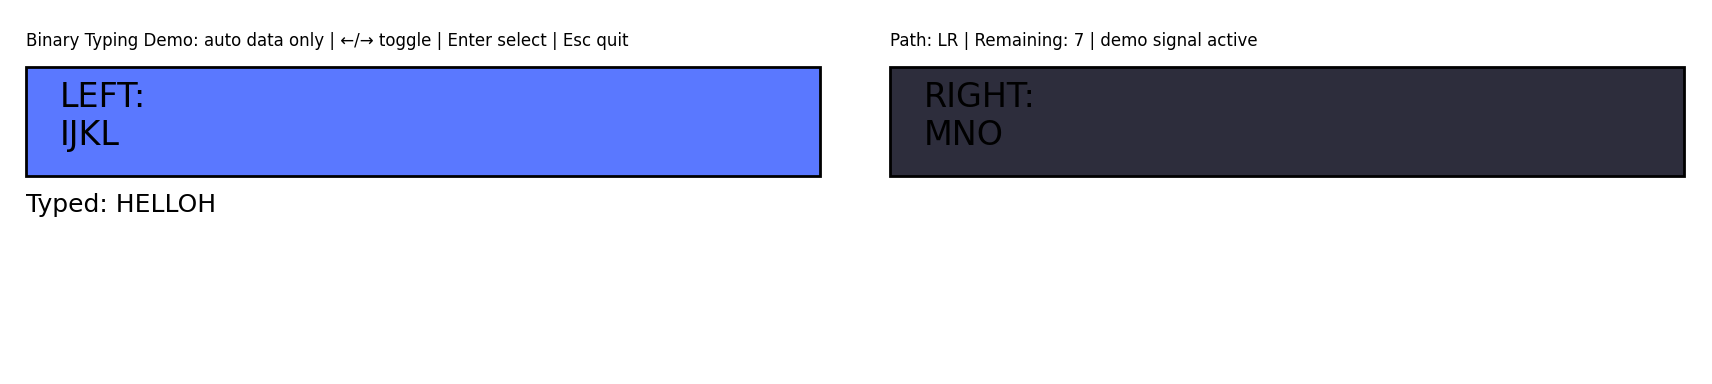
\includegraphics[width=\textwidth]{src/images/figures/keyboard_2.png}
	\caption{Keyboard Interface}
	\label{keyboard_2}
\end{figure}

\newpage
\section{Code Snippets}
\subsection{Keyboard Interface Code Snippet:}


\lstset{
	basicstyle=\ttfamily\footnotesize,
	frame=none,
	numbers=none,
	breaklines=true,
	columns=fullflexible,
	showstringspaces=false,
	keepspaces=true,
	tabsize=4,	
	backgroundcolor=\color{white},
	xleftmargin=0pt,
	framexleftmargin=0pt,
	keywordstyle=\relax,
	commentstyle=\relax,
	stringstyle=\relax,
	literate=
	{←}{{$\leftarrow$}}1
	{→}{{$\rightarrow$}}1
	{…}{{\ldots}}1
}

\begin{lstlisting}[language=Python]
	SYMBOLS = "ABCDEFGHIJKLMNOPQRSTUVWXYZ _<"
	
	class BinaryTyper:
	def __init__(self, symbols: str):
	self.all_symbols = list(symbols)
	self.reset_group()
	self.highlight = 0
	self.typed = ""
	
	def reset_group(self):
	self.group = self.all_symbols[:]
	self.path = []
	
	def split(self):
	mid = (len(self.group) + 1) // 2
	left = self.group[:mid]
	right = self.group[mid:]
	return left, right
	
	def toggle(self):
	self.highlight = 1 - self.highlight
	
	def select(self):
	left, right = self.split()
	chosen = left if self.highlight == 0 else right
	
	self.group = chosen
	self.path.append("L" if self.highlight == 0 else "R")
	self.highlight = 0
	
	if len(self.group) == 1:
	sym = self.group[0]
	
	if sym == "_":
	self.typed += " "
	elif sym == "<":
	self.typed = self.typed[:-1]
	else:
	self.typed += sym
	
	self.reset_group()
	
	def backspace(self):
	self.typed = self.typed[:-1]
	
	def previews(self):
	left, right = self.split()
	return left, right, len(self.group), "".join(self.path)
\end{lstlisting}


\lstdefinestyle{ArduinoStyle}{
	backgroundcolor=\color{white},   % white background for printing
	basicstyle=\ttfamily\footnotesize,
	keywordstyle=\color{codeblue}\bfseries,
	commentstyle=\color{codegreen}\itshape,
	stringstyle=\color{red},
	numbers=left,
	numberstyle=\tiny\color{codegray},
	stepnumber=1,
	numbersep=5pt,
	showstringspaces=false,
	breaklines=true,
	frame=none,
	captionpos=b
}

\subsection{Interrupt Service Setup and Routine}

\begin{lstlisting}[style=ArduinoStyle, language=C, caption={Interrupt Service Setup and Routine in Arduino for Sampling}, label={isr}]
	void setupTimer1_1024Hz(){
		cli();
		TCCR1A = 0;
		TCCR1B = 0;
		OCR1A = 31249;       // 16MHz -> 512Hz
		TCCR1B = 0x09;       // prescaler=1
		TIMSK1 = 0x02;       // enable OCR1A interrupt
		sei();
	}
	
	ISR(TIMER1_COMPA_vect){
		ADCSRA |= (1 << ADSC); 
		float sample = adc * ADC;
		sample-=5;
		
		circBuf[writeIndex] = sample;
		writeIndex = (writeIndex + 1) & (N - 1);
		
		samplesCollected++;
		if (samplesCollected >= N &&
		(((samplesCollected - N) & (HOP_SIZE - 1)) == 0)) {
			fftReady = true;
		}
	}
\end{lstlisting}

\newpage
\subsection{Code Snippet of FFT on Arduino}
\begin{lstlisting}[style=ArduinoStyle, language=C, caption={FFT Function}, label={fft}]
	void fft(float *real, float *imag){
		bitReversalPermutation(real, imag);
		
		for (uint8_t stage = 1; stage <= 7; stage++){
			uint8_t m = 1 << stage;
			uint8_t m2 = m >> 1;
			
			float theta = -2.0 * PI / m;
			float wm_real = fastCos(theta);
			float wm_imag = fastSin(theta);
			
			for (uint8_t k = 0; k < N; k += m){
				float w_real = 1.0;
				float w_imag = 0.0;
				
				for (uint8_t j = 0; j < m2; j++){
					uint8_t t = k + j + m2;
					uint8_t u = k + j;
					
					float tr = w_real * real[t] - w_imag * imag[t];
					float ti = w_real * imag[t] + w_imag * real[t];
					
					real[t] = real[u] - tr;
					imag[t] = imag[u] - ti;
					
					real[u] += tr;
					imag[u] += ti;
					
					// w = w * wm
					float temp = w_real;
					w_real = temp * wm_real - w_imag * wm_imag;
					w_imag = temp * wm_imag + w_imag * wm_real;
				}
			}
		}
	}
\end{lstlisting}
